\documentclass[a4paper,12pt]{article}
\usepackage[a4paper, margin=2.5cm]{geometry}
\usepackage[pdftex]{graphicx}
\usepackage{tikz}
\usepackage{pgfplots}
\usepackage{enumitem}
\usepackage{float}
\usepackage[document]{ragged2e}
\usepackage[utf8]{inputenc}
\usepackage[T1]{fontenc}
\usepackage[spanish,es-tabla]{babel}
\renewcommand{\shorthandsspanish}{}
\usepackage{xurl}
\usepackage{lipsum}
\usepackage{mwe}
\usepackage{multirow}
\usepackage{multicol}
\usepackage{siunitx}
\usepackage{listings}
\usepackage{circuitikz}
\usepackage{tabularray}
\usepackage{amsmath}
\usepackage{gensymb}


\usetikzlibrary{arrows.meta,bending}
\graphicspath{ {/home/saikkopat/Documents/ESCOM/FDD/P02/IMG/} }

\usepackage[none]{hyphenat}

\begin{document}

\begin{titlepage}
	\begin{tikzpicture}[overlay, remember picture]
		\path (current page.north east) ++(-0.3,-1.8) node[below left] {
\includegraphics[width=0.35\textwidth]{/home/saikkopat/Documents/LOGOS IPN/EscudoESCOM}};
	\end{tikzpicture}
	\begin{tikzpicture}[overlay, remember picture]
		\path (current page.north west) ++(1.5,-1) node[below right] {
\includegraphics[width=0.2\textwidth]{/home/saikkopat/Documents/LOGOS IPN/logo}};
	\end{tikzpicture}
	\begin{center}
		\vspace{-1.5cm}
		{\LARGE Instituto Politécnico Nacional\par}
		\vspace{.5cm}
		{\LARGE Escuela Superior de Cómputo\par}
		\vspace{.5cm}
		{\Large Departamento de\\Ingeniería en Sistemas Computacionales\par}
		\vspace{2cm}
		{\large Unidad de aprendizaje:}\\{\Large Fundamentos de diseño digital\par}
		\vspace{2cm}
		{\scshape\Huge Práctica 2\par}
		{\itshape\Large Minimización algebraica\par}
		\vfill
		\vspace{.7cm}
		{\Large Equipo 2\par}
		\vspace{.7cm}
		{\Large Grupo: 3CV2\par}
		\vspace{.7cm}
		{\Large Integrantes:\\González Cárdenas Ángel Aquilez\\Hernández Reyes Diego Alberto\par}
		\vspace{1cm}
		{\Large Profesor: Barrón Vera Josué Emanuel\par}
		\vspace{1cm}
		{\large Fecha de realización: 19 de septiembre de 2023\par}
		{\large Fecha de entrega: 25 de septiembre de 2023\par}
		\vfill
	\end{center}
\end{titlepage} 

\newpage

\tableofcontents

\newpage

\usepgfplotslibrary{units}

En el presente reporte de laboratorio correspondiente a la segunda práctica, se aborda el diseño y la verificación de un comparador con magnitud de dos bits, así como el diseño y simplificación de un generador de código Gray para cuatro bits.\par 

\section*{Objetivo}

\textbf{Objetivo}: Al terminar la sesión, los integrantes del equipo contarán con la habilidad de diseñar circuitos combinatorios a partir de un enunciado.\par

\vspace{.5cm}

Los alumnos utilizarán los siguientes materiales y equipo:

\begin{multicols}{2}
\textbf{Equipo}\\
\begin{itemize}[nosep]
		\item 10 \texttt{LEDS} de colores
		\item \texttt{Dip switch}
		\item Fuente de Alimentación
		\item Manual de especificaciones \textit{FAST and LS TTL} de MOTOROLA\textregistered
\end{itemize}

\columnbreak

\textbf{Material}\\
\begin{itemize}[nosep]
		\item \textit{Protoboard}
		\item 1 C. I. 74LS00
		\item 1 C. I. 74LS02
		\item 1 C. I. 74LS04
		\item 1 C. I. 74LS08
		\item 1 C. I. 74LS32
		\item 1 C. I. 74LS86
	
\end{itemize}

\end{multicols}


%
%
%		DESAROLLO
%
%

\section{Desarrollo}

\subsection{Comparador de dos bits}

El comparador de dos bits se caracteriza por poseer dos entradas ($A, B$) y tres salidas correspondientes a las operaciones $A < B$, $A = B$ y $A > B$.\par

La Figura 1 ilustra la tabla de verdad que indica los valores para los cuales son verdaderas las operaciones.\par

\begin{figure}[ht!]
	\centering

	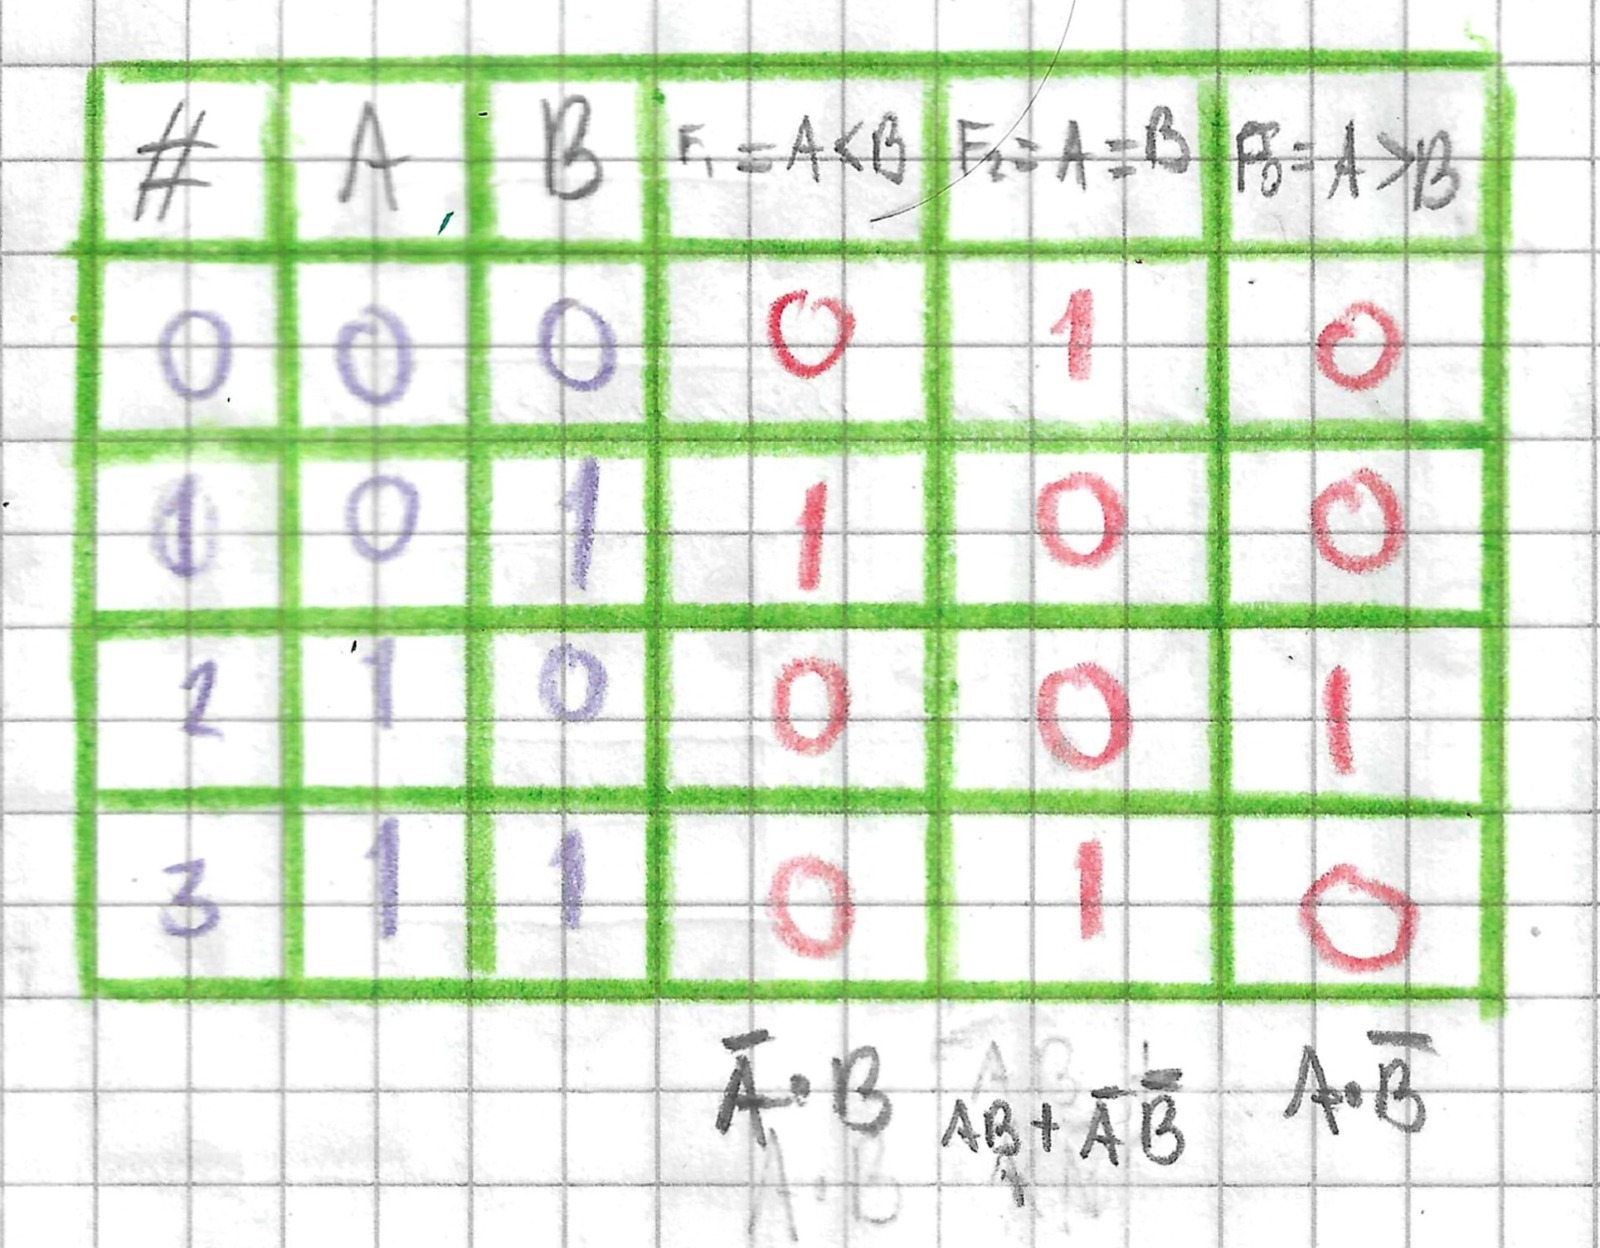
\includegraphics[width=.65\textwidth]{T01}

	\caption{Tabla de verdad del comparador de dos bits}
\end{figure}

Después, con los valores para los cuales las salidas producen un valor alto, o verdadero, se determina qué operación produce el resultado deseado realizando la suma de productos correspondiente.\par

Para $F_1$ (que se produce por la operación $A < B$), es verdadera solo cuando $A$ es un valor bajo y $B$ un valor alto. De modo que la expresión que nos entregará el resultado deseado será:\par

\[ \overline{\rm A}B \]\par

De manera análoga para $F_2$ tenemos:

\[ AB + \overline{\rm A} (\overline{\rm B}) \]\par

Y para $F_3$

\[ A\overline{\rm B} \]\par


Una vez determinadas las expresiones que otorgan los resultados correctos, se obtuvieron los siguientes circuitos lógicos:\par

\vspace{1cm}

\begin{figure}[ht!]
	\centering

	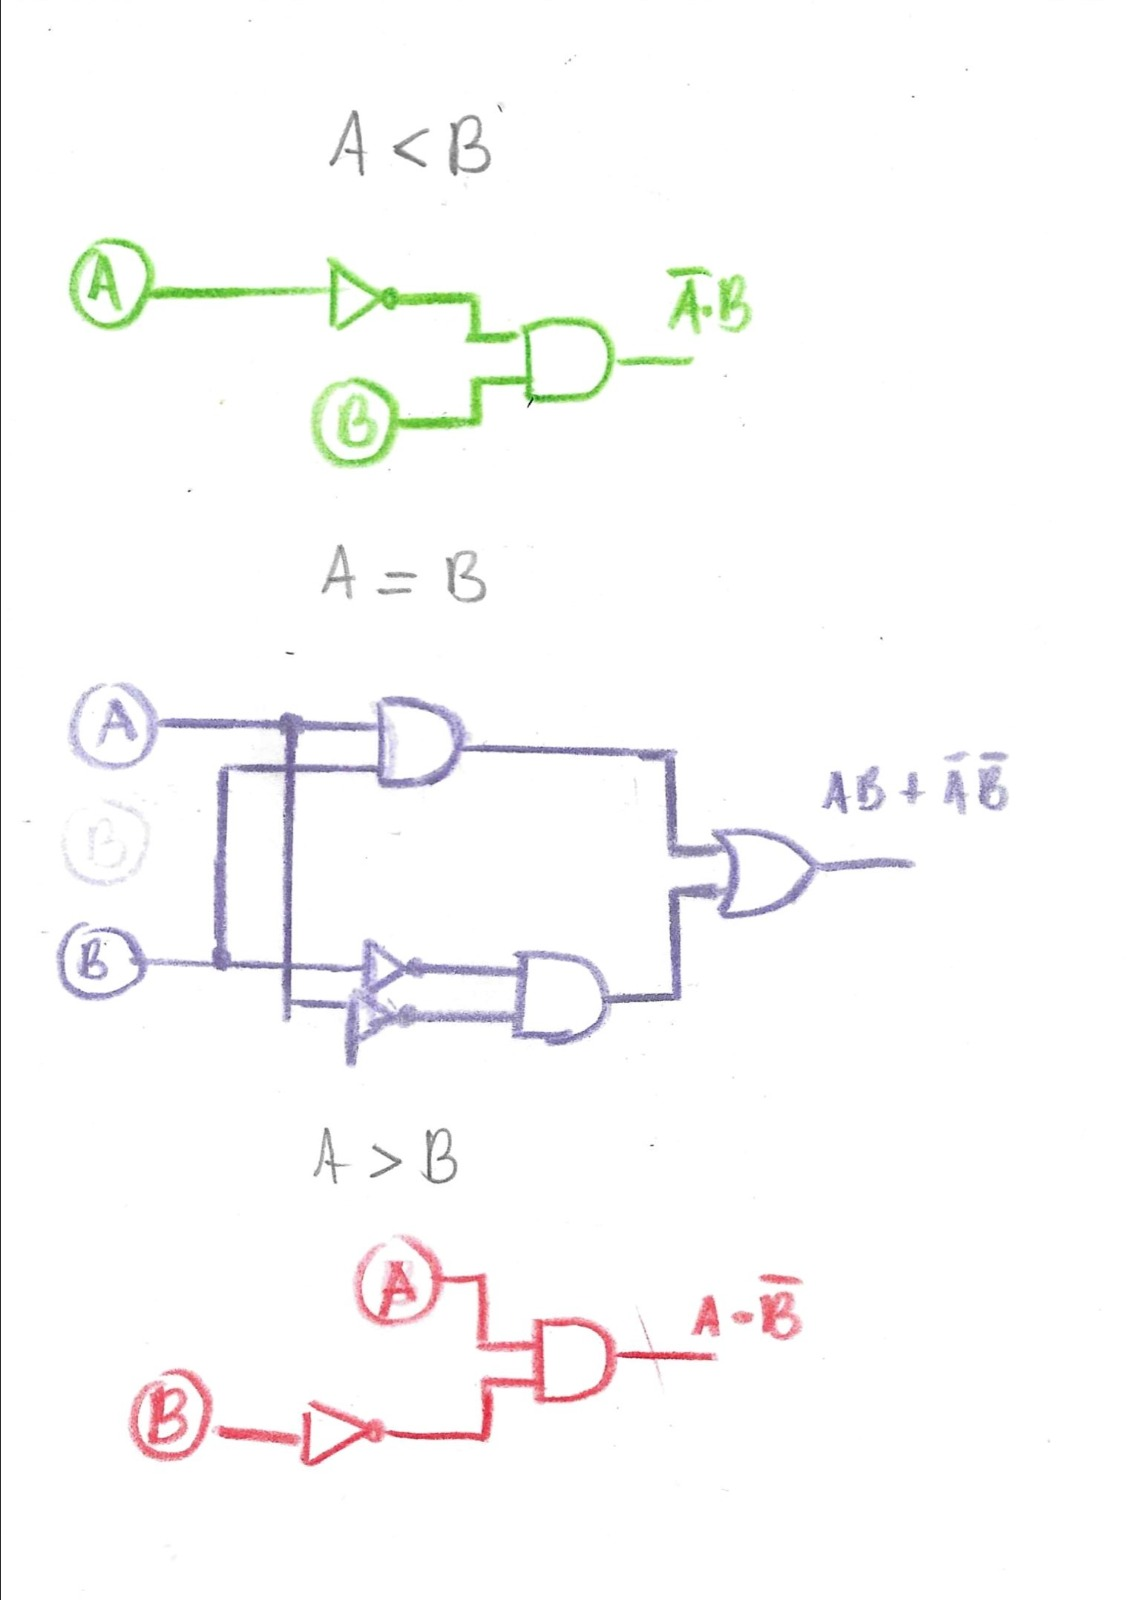
\includegraphics[width=.5\textwidth]{C01}

	\caption{Circuitos lógicos del comparador de dos bits}
\end{figure}


Por consiguiente, el circuito en funcionamiento se muestra en las Figuras 3 y 4:\par

\begin{figure}[ht!]
	\centering

	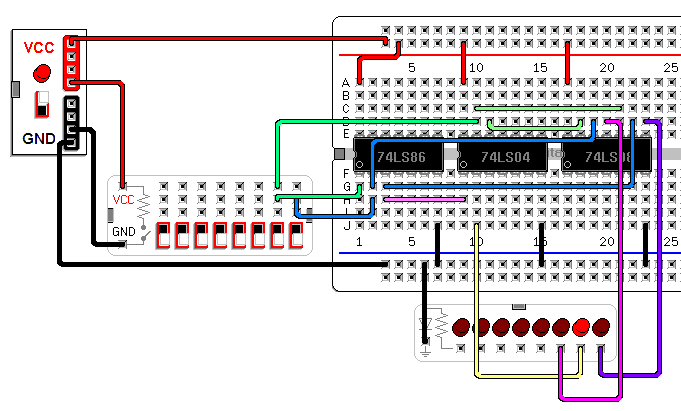
\includegraphics[width=.7\textwidth]{S01}

	\caption{Circuito comparador $A = 0, B = 0, F_2 = 1$}
\end{figure}

\begin{figure}[ht!]
	\centering

	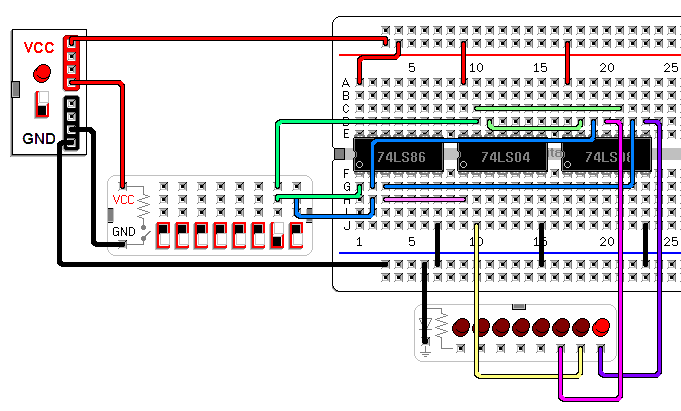
\includegraphics[width=.7\textwidth]{S02}

	\caption{Circuito comparador $A = 1, B = 0, F_3 = 1$}
\end{figure}

\begin{figure}[ht!]
	\centering

	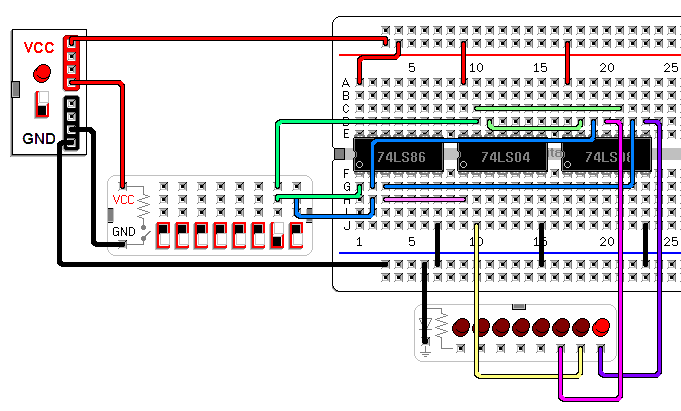
\includegraphics[width=.7\textwidth]{S02}

	\caption{Circuito comparador $A = 1, B = 1, F_2 = 1$}
\end{figure}

\newpage



\subsection{Generador de código Grey de cuatro bits}

\vspace{1cm}


La principal característica del código Grey es el cambio en solo un bit entre la salida anterior y la siguiente, que se puede apreciar en la tabla de verdad correspondiente al código Grey para cuatro entradas de la Figura 6:\par

\vspace{1cm}

\begin{figure}[ht!]
	\centering

	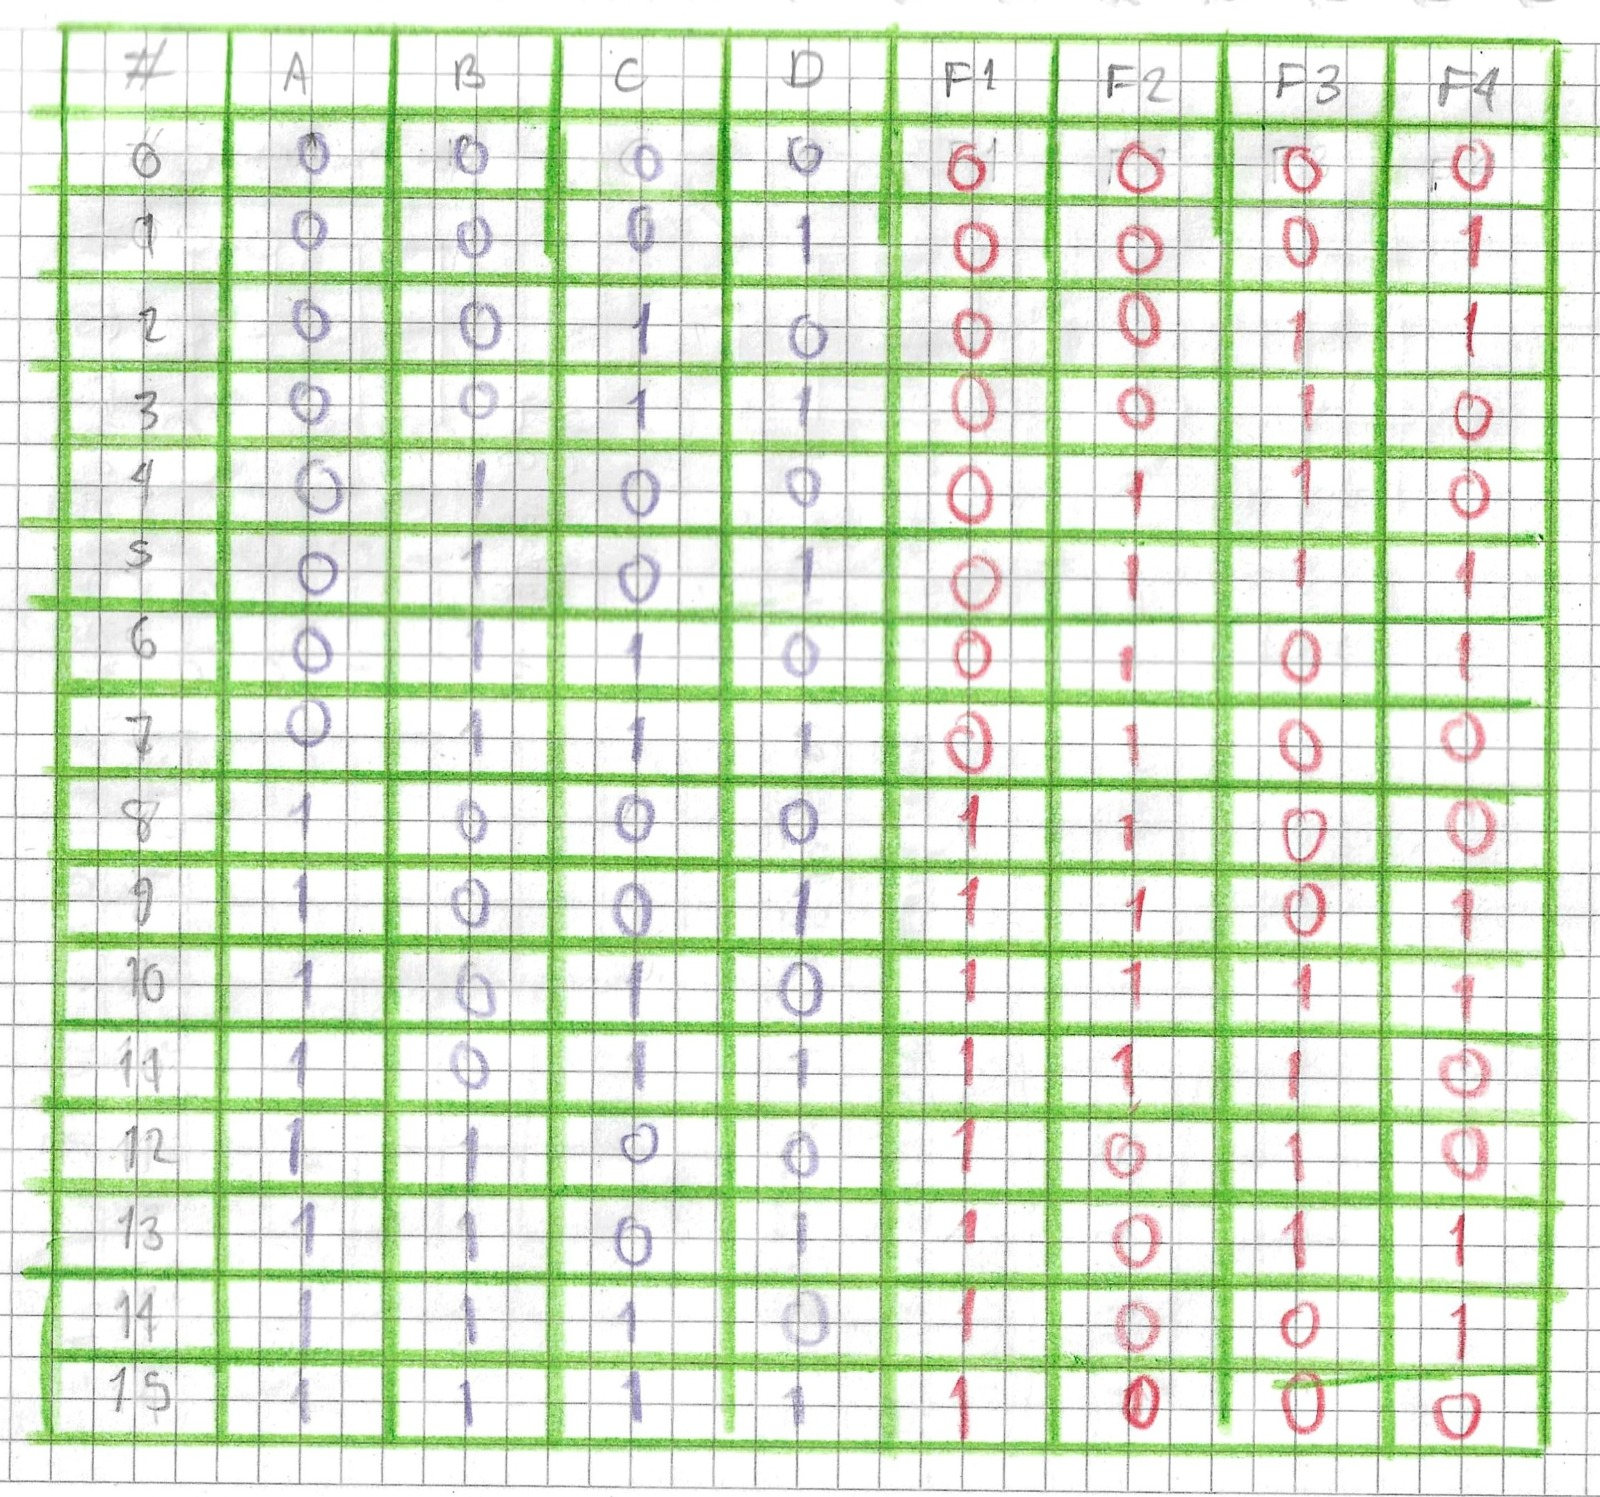
\includegraphics[width=.85\textwidth]{T02}

	\caption{Tabla de verdad del código Grey}
\end{figure}

\vspace{1cm}

De manera similar al ejercicio anterior, se obtiene la suma de productos para los cuales la salida es positiva, esto es: la suma de minterminos. Como las salidas son cuatro, se obtuvieron cuatro enunciados distintos, lo que significa cuatro circuitos independientes entre sí.\par

\vspace{1cm}

Por simple inspección, se aprecia que la salida para $F_1$ será equivalente a los valores de entrada para $A$, lo cual se comprueba en la Figura 7 que muestra la simplificación realizada:\par

\begin{figure}[ht!]
	\centering

	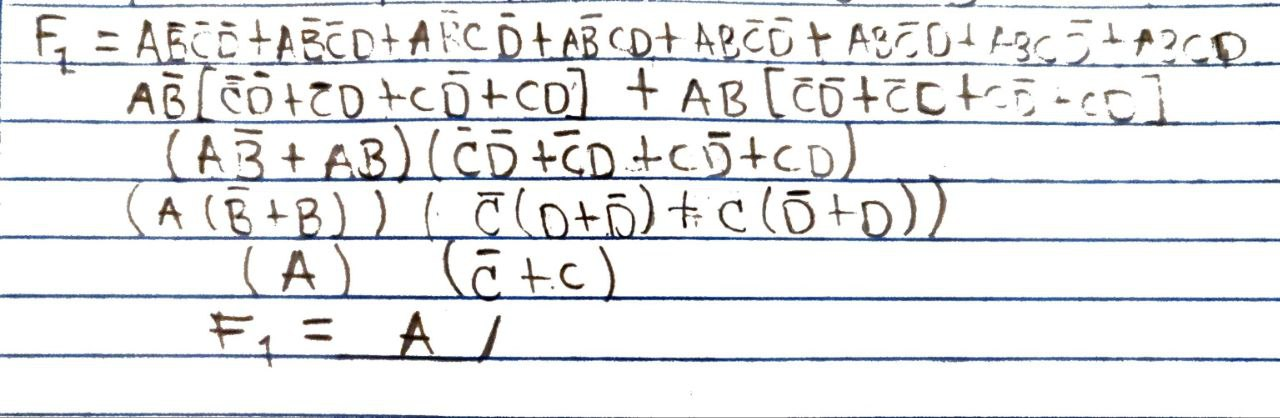
\includegraphics[width=.75\textwidth]{F1}

	\caption{Simplificación para $F_1$}
\end{figure}

La principal motivación para realizar la simplificación se encuentra en la reducción de componentes a utilizar cuando se construyen los circuitos, como se puede ver en la Figura 8 al reducirse drásticamente el número de componentes:\par


\begin{figure}[ht!]
	\centering

	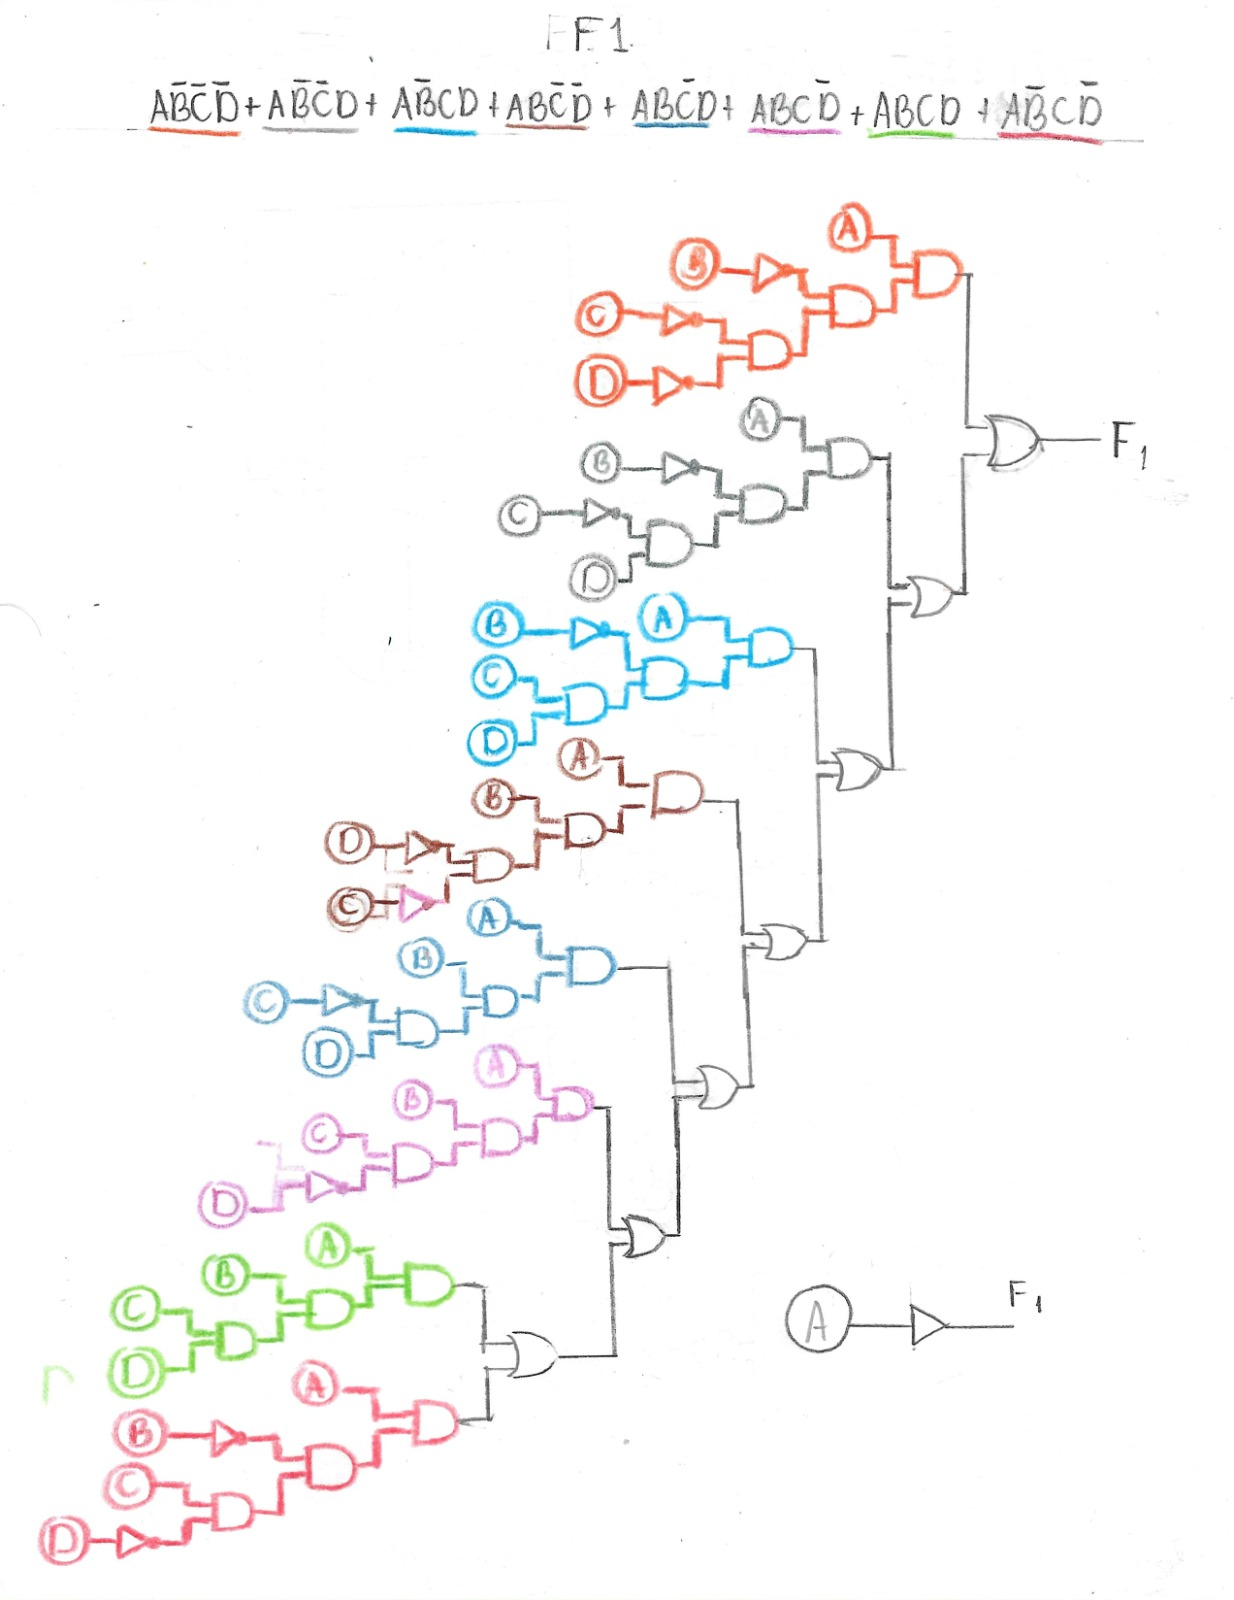
\includegraphics[width=.75\textwidth]{CF1}

	\caption{Simplificación para el circuito de $F_1$}
\end{figure}

\newpage

De manera análoga, se determinan la suma de mintérminos para cada salida y se simplifican a su mínima expresión equivalente.\par

\begin{figure}[ht!]
	\centering

	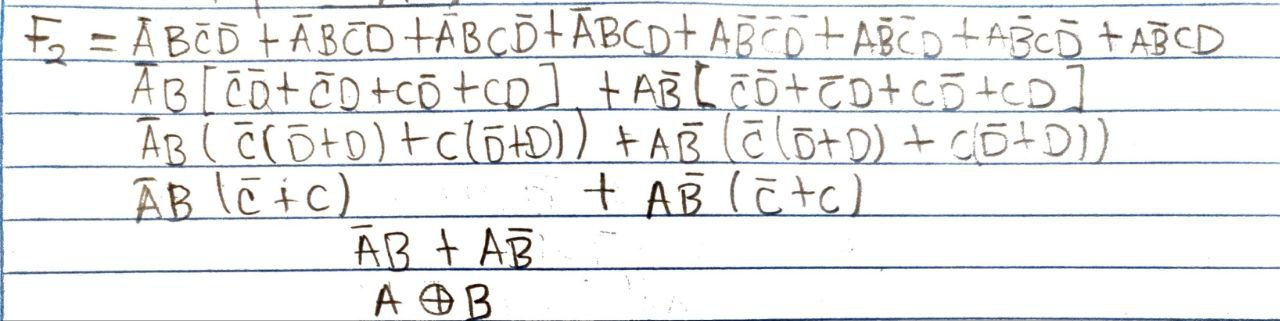
\includegraphics[width=.75\textwidth]{F2}

	\caption{Simplificación para $F_2$}
\end{figure}

\vspace{1cm}

\begin{figure}[ht!]
	\centering

	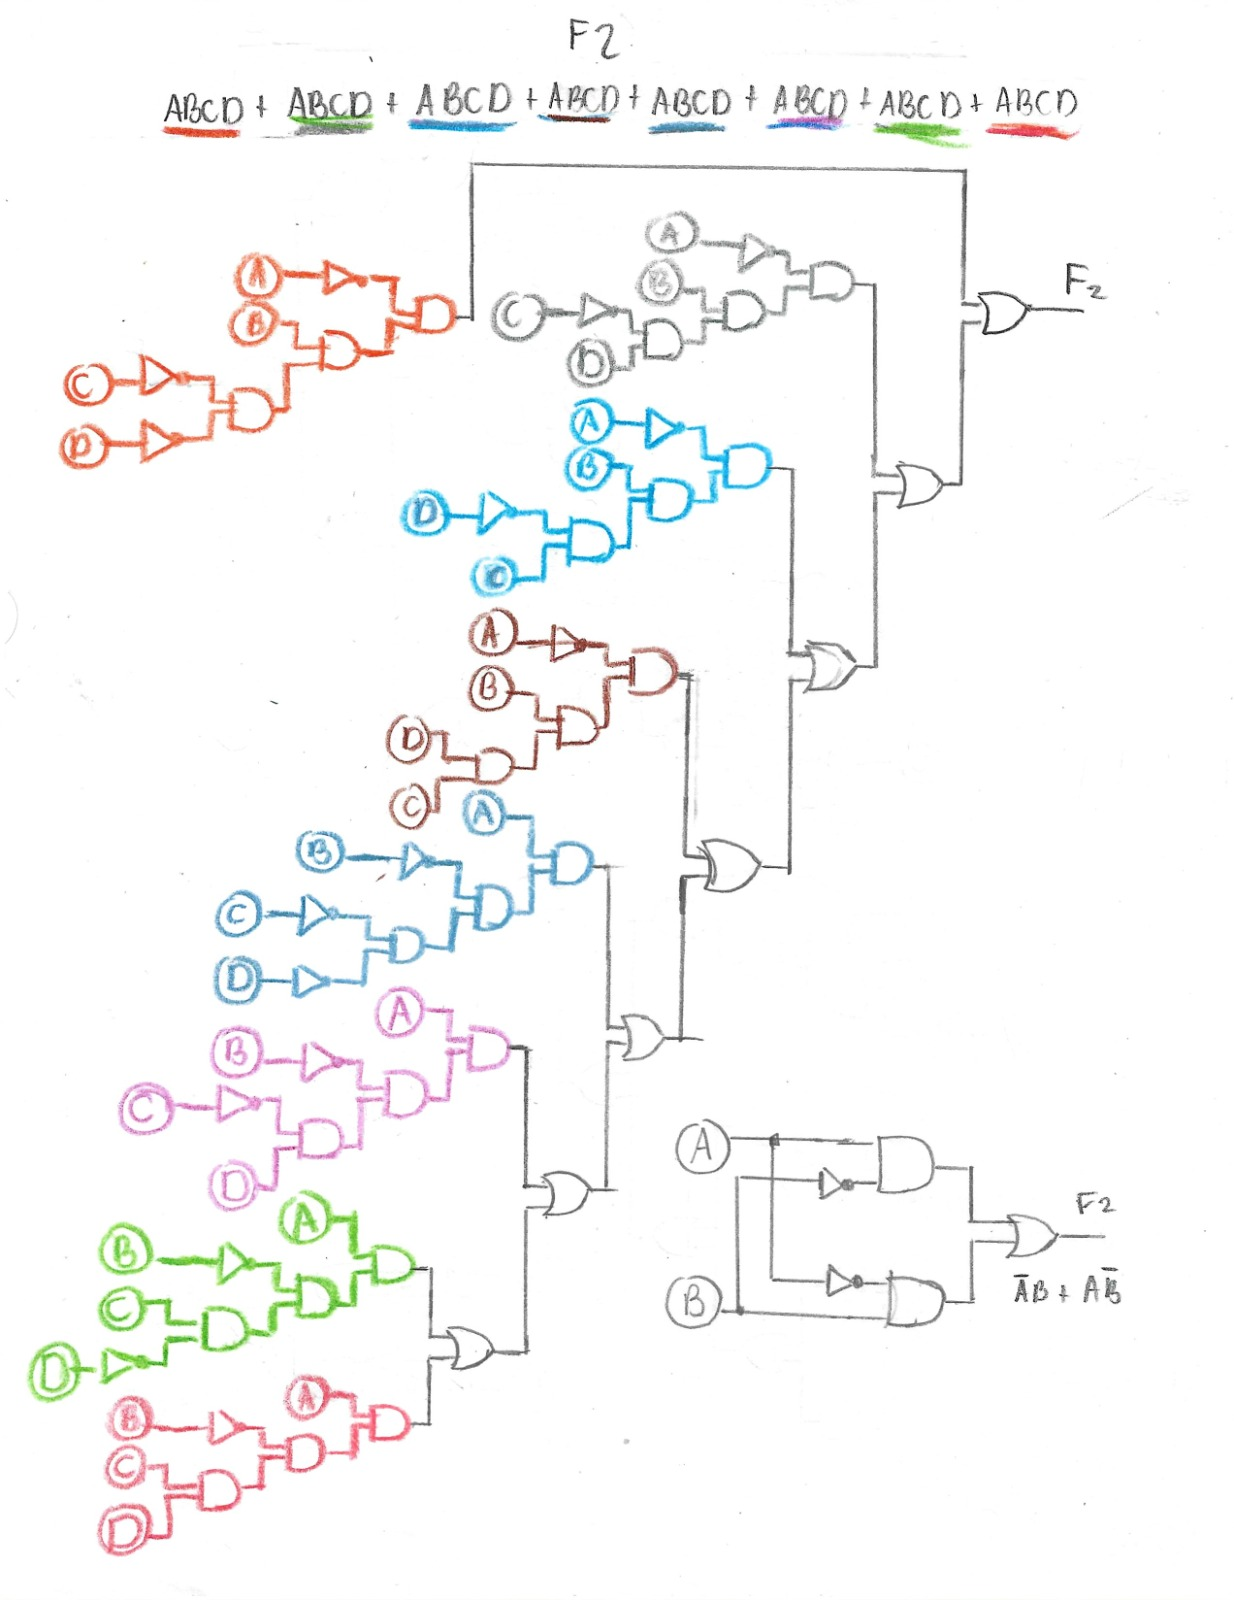
\includegraphics[width=.75\textwidth]{CF2}

	\caption{Simplificación para el circuito de $F_2$}
\end{figure}

\newpage

\begin{figure}[ht!]
	\centering

	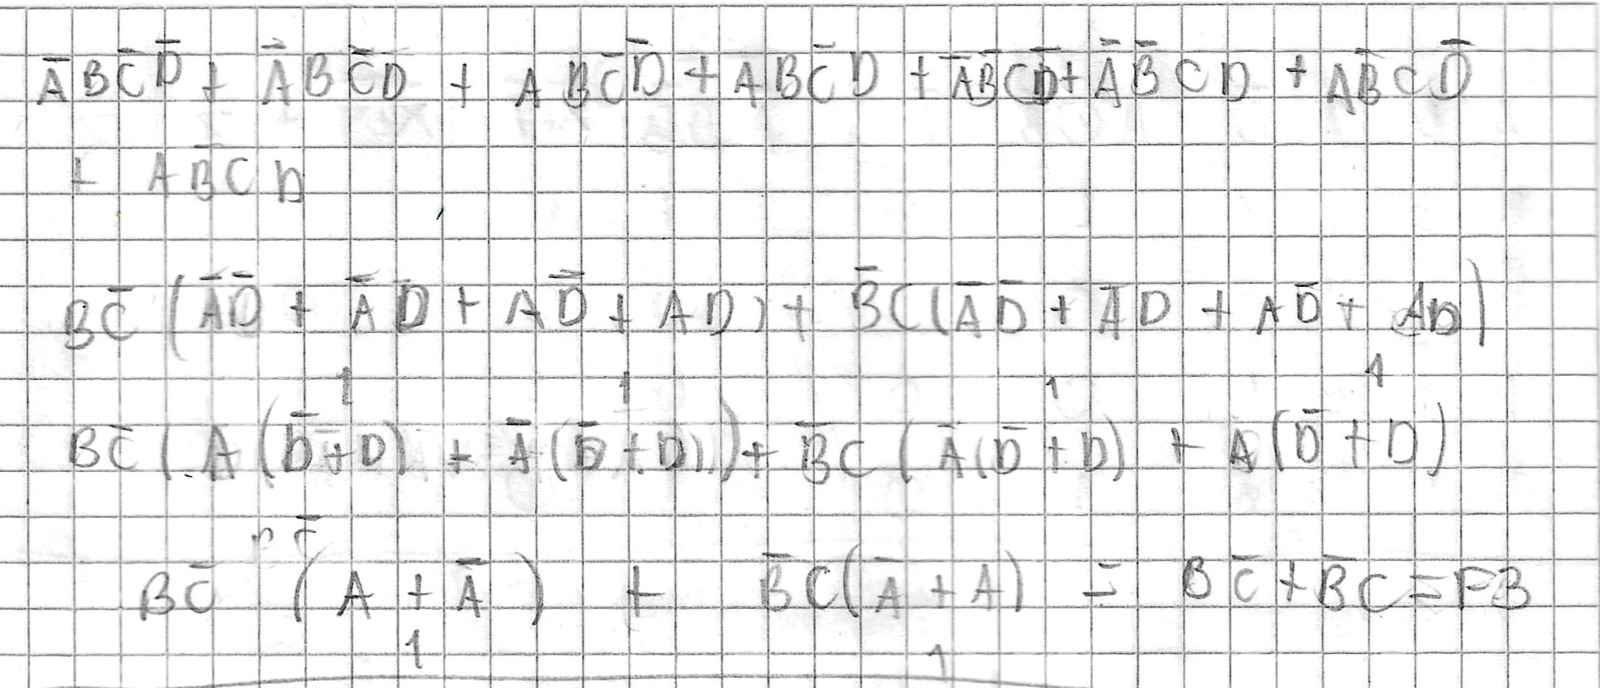
\includegraphics[width=.75\textwidth]{F3}

	\caption{Simplificación para $F_3$}
\end{figure}

\vspace{1cm}

\begin{figure}[ht!]
	\centering

	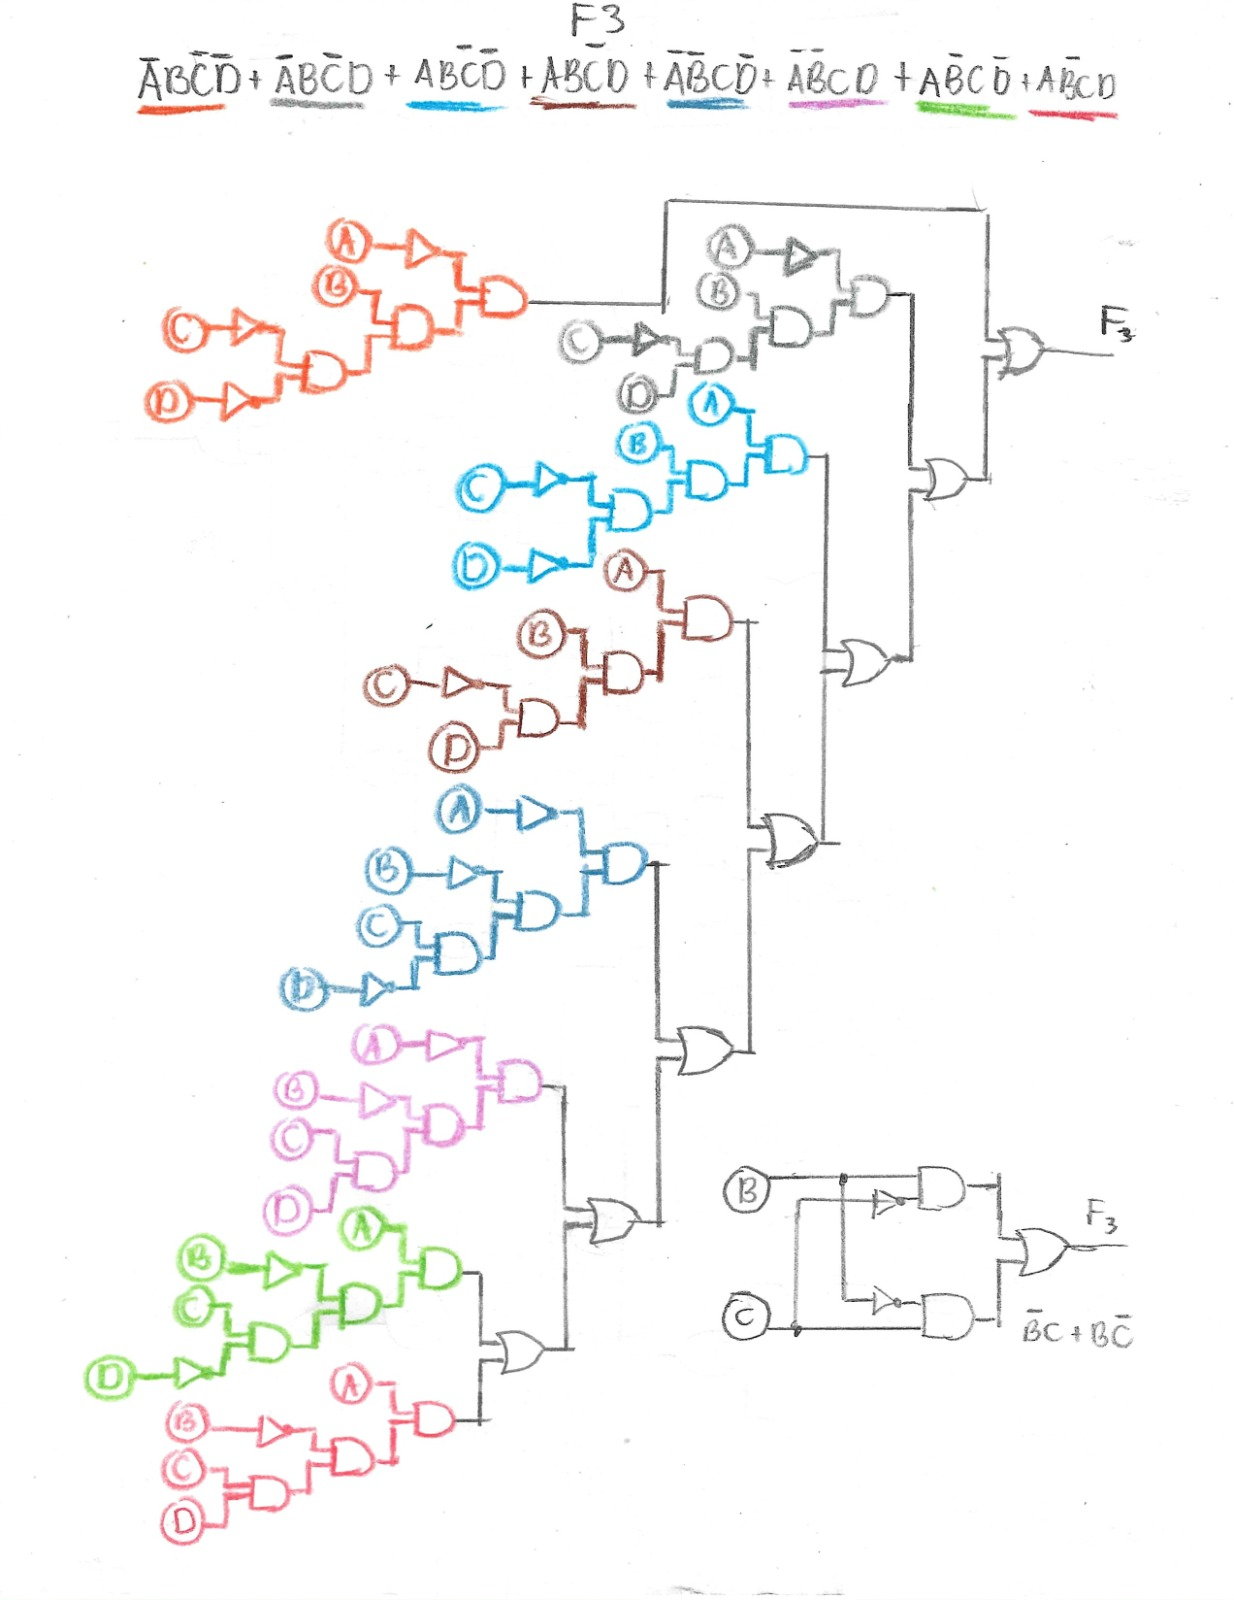
\includegraphics[width=.75\textwidth]{CF3}

	\caption{Simplificación para el circuito de $F_3$}
\end{figure}

\newpage

\begin{figure}[ht!]
	\centering

	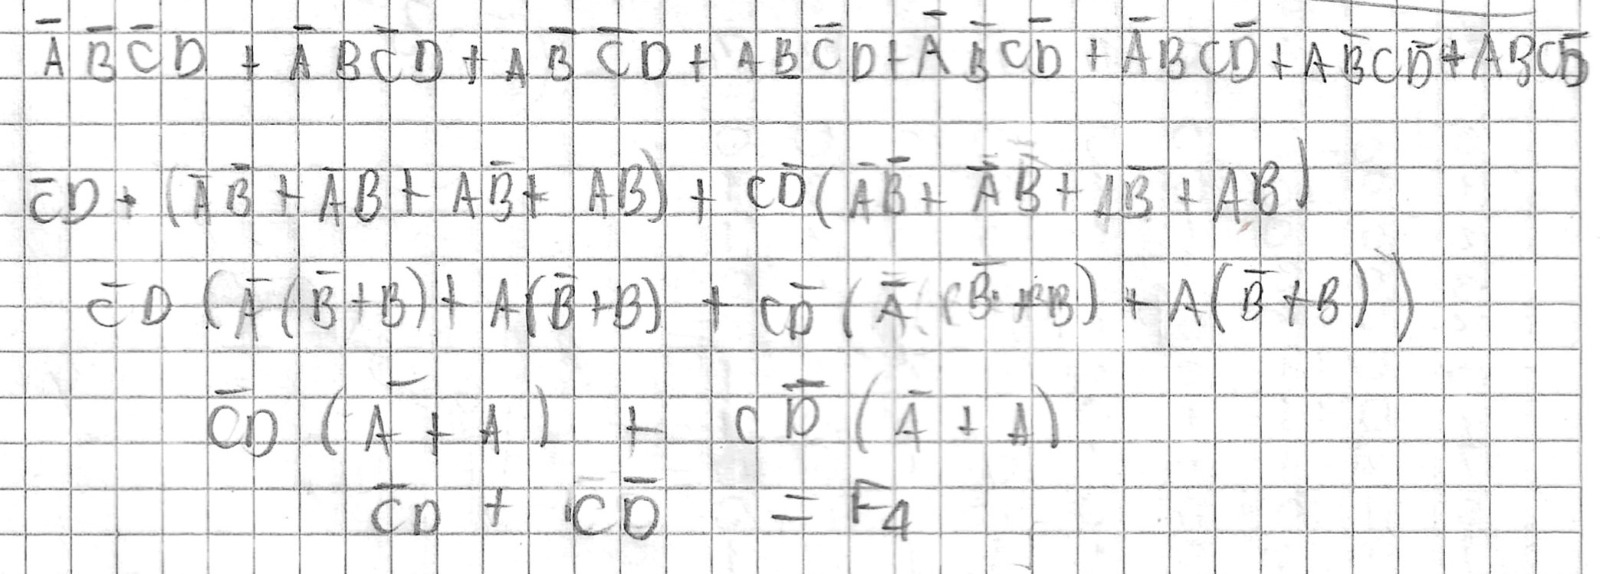
\includegraphics[width=.75\textwidth]{F4}

	\caption{Simplificación para $F_4$}
\end{figure}

\vspace{1cm}

\begin{figure}[ht!]
	\centering

	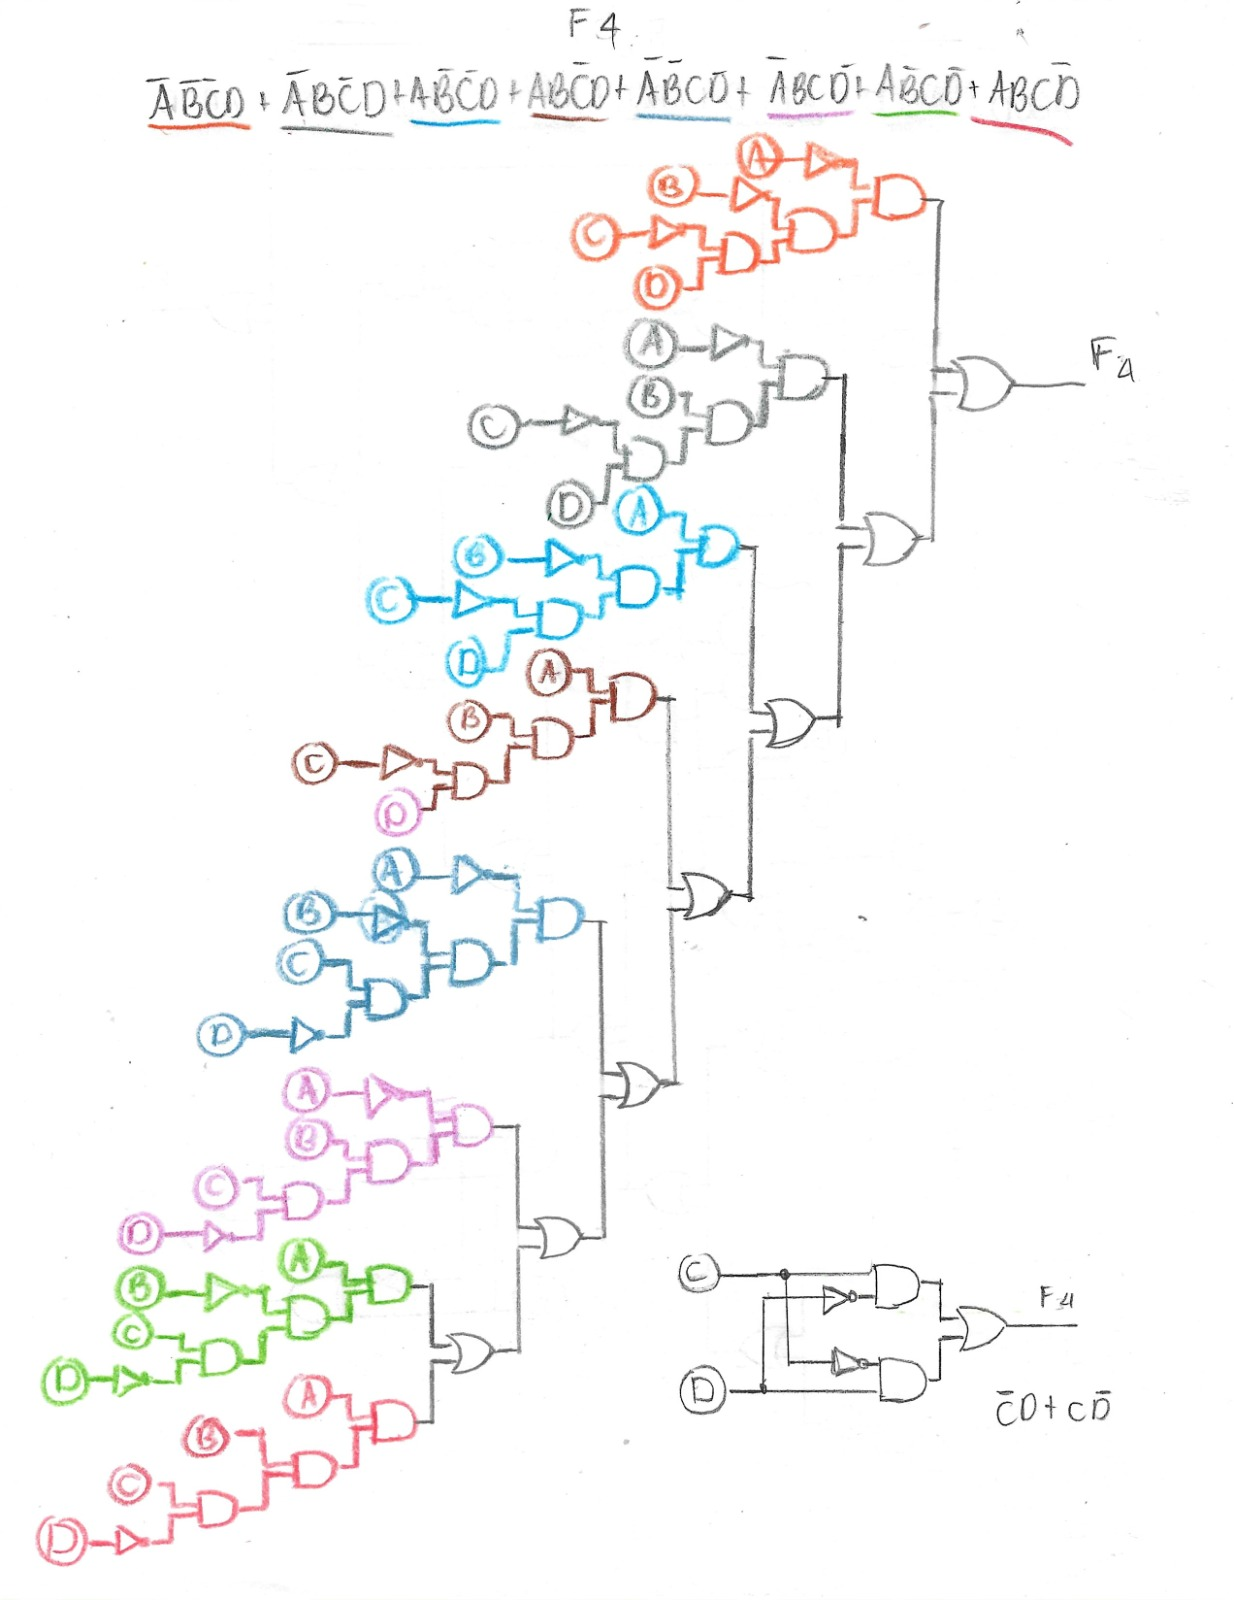
\includegraphics[width=.75\textwidth]{CF4}

	\caption{Simplificación para el circuito de $F_4$}
\end{figure}



\newpage

Una vez obtenidos los equivalentes simplicados se procedió a construir el circuito, que se aprecia en la Figura 15:


\begin{figure}[ht!]
	\centering

	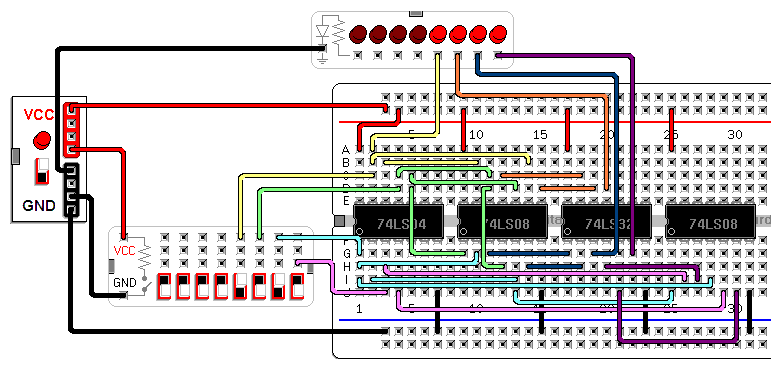
\includegraphics[width=.7\textwidth]{GR1}

	\caption{$A=1, B=0, C=1,D=0$, Equivalente Grey: 1111}
\end{figure}

Este primer circuito fue construido a partir de las expresiones simplificadas sin hacer uso de la compuerta \emph{XOR}.\par


\begin{figure}[ht!]
	\centering

	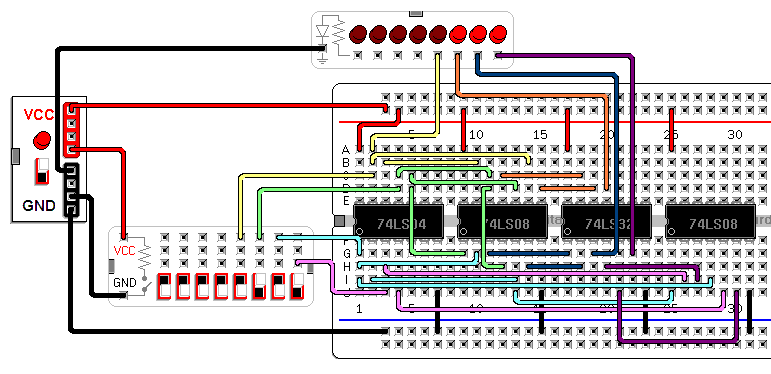
\includegraphics[width=.7\textwidth]{GR2}

	\caption{Entrada: 0101, Grey: 1111}
\end{figure}

\begin{figure}[ht!]
	\centering

	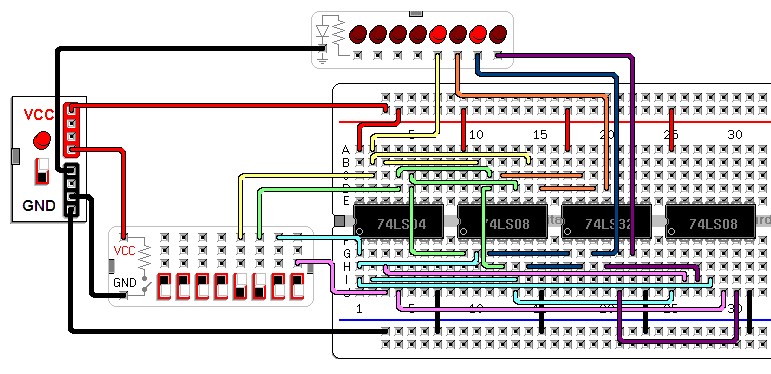
\includegraphics[width=.7\textwidth]{GR3}

	\caption{Entrada: 1100, Grey: 1010}
\end{figure}

\newpage

Ahora, utilizando una compuesta \emph{XOR} y sus equivalentes para cada salida, se obtuvo el siguiente circuito:\par

\begin{figure}[ht!]
	\centering

	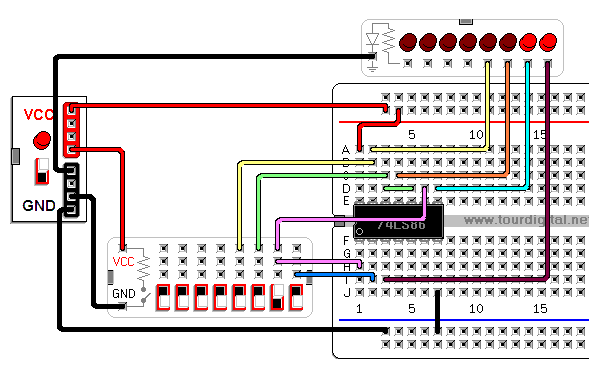
\includegraphics[width=.8\textwidth]{GR4}

	\caption{Entrada: 0010, Grey: 0011}
\end{figure}

Se vuelve evidente la importancia de la simplificación y el ahorro de componentes en comparación con las expresiones donde solo se utilizaron \emph{AND}, \emph{OR} y \emph{NOT}.\par

\begin{figure}[ht!]
	\centering

	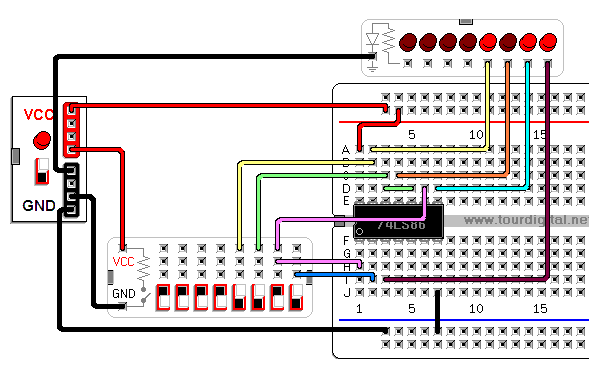
\includegraphics[width=.8\textwidth]{GR5}

	\caption{Entrada: 1101, Grey: 1011}
\end{figure}



\newpage
%
%
%		CONCLUSIONES
%
%

\section{Observaciones y conclusiones}

González Cárdenas Ángel Aquilez

\begin{quotation}
	La práctica de laboratorio involucró la construcción de un circuito comparador de dos bits y un generador de código Gray de cuatro bits, los cuales destacaron la importancia de la simplificación en el diseño de circuitos lógicos y el ahorro que esto puede representar en términos del número de compuertas utilizadas. \par

	Primero, se obtuvo la tabla de verdad de cada circuito y se extrajeron los minterminos de las expresiones lógicas correspondientes. Posteriormente, se llevó a cabo la simplificación de estas expresiones a su forma más reducida. Este paso de simplificación es crítico en el diseño de circuitos digitales, ya que permite reducir la complejidad y la cantidad de componentes necesarios para implementar una función lógica.\par

	El ahorro que se logra a través de la simplificación es de gran importancia tanto en términos de costos como de eficiencia. Menos compuertas lógicas significa menos componentes electrónicos, menos espacio físico requerido y, en última instancia, menor consumo de energía. Además, la simplificación conlleva una mejora en la velocidad de operación del circuito, ya que menos compuertas implican menos retardos en la señal.\par

	Al concluir la práctica, se demostró la importancia de la simplificación en el diseño de circuitos digitales, resaltando cómo la optimización de las expresiones lógicas puede llevar a un ahorro significativo en términos de recursos.\par
\end{quotation}

\vspace{1cm}

Hernández Reyes Diego Alberto

\begin{quotation}
	Al concluir la práctica, se construyeron los circuitos de un circuito comparador de dos bits y un generador de código Gray de cuatro bits. Se resaltó la importancia de construir circuitos a partir de expresiones simplificadas para lograr un diseño eficiente y confiable.\par

	En este proceso, al simplificar las expresiones lógicas de cada salida, se obtuvo una representación más clara y compacta de las funciones que debían ser implementadas en los circuitos. Al construir los circuitos basándose en estas expresiones simplificadas, se logra una serie de ventajas:\par

	\begin{itemize}
		\item Mayor confiabilidad: Las expresiones simplificadas reducen la probabilidad de errores en la implementación física, ya que implican menos puertas lógicas y, por lo tanto, menos posibilidades de fallos.
		\item Eficiencia de recursos: Al construir circuitos a partir de expresiones simplificadas, se utiliza un número menor de componentes electrónicos, lo que resulta en un uso más eficiente de los recursos y reduce los costos de producción.
		\item Facilita el mantenimiento: Los circuitos basados en expresiones simplificadas son más fáciles de mantener y depurar, ya que la lógica subyacente es más clara y comprensible.
		\item Mejora el rendimiento: La simplificación de las expresiones lógicas puede conducir a un menor retardo en el circuito, lo que se traduce en un mejor rendimiento y tiempos de respuesta más rápidos.
		\item Ahorro de energía: Menos compuertas lógicas en el circuito implican un menor consumo de energía, lo que es especialmente importante en aplicaciones de bajo consumo energético.
	\end{itemize}

	En conclusión, la construcción de circuitos a partir de expresiones simplificadas es esencial para lograr diseños de circuitos digitales eficientes, confiables y rentables. Esta práctica subrayó la importancia de la simplificación como una herramienta fundamental, permitiendo la implementación de circuitos más efectivos y robustos.\par
\end{quotation}

\end{document}